\section{Heuristic Evaluation and Weight Determination}

To evaluate the effectiveness of our heuristics and to determine suitable weights for score calculation in both Min-Max and Alpha-Beta Pruning, we conducted a detailed analysis of each heuristic.\\
To find good weights, we automated the process. The corresponding code can be found in the "Heuristic-Eval" branch. We created a shell script to run client vs AI games for every weight combination specified in our input file. The results were stored in a results file and visualized using a Python script.\\
Let us first examine the individual heuristics. \textbf{Stones} refers to the percentage of the player's stones relative to the total on the board. \textbf{Walls} indicates the number of walls adjacent to the player's pieces. \textbf{Enemies} represents the number of opponents adjacent to the player's pieces. \textbf{Overrides} indicates the difference in override stones compared to the opponent (for example, -1 means the player has one fewer override stone).\\
As one might notice, these are only 4 heuristics. This is because the runtime and complexity of our fifth heuristic was to great and we chose to give up on it. Although we have some ideas for the fifth heuristic, there was nothing we were truly happy with, As such this examination will only treat four heuristics.

\begin{figure}[H]
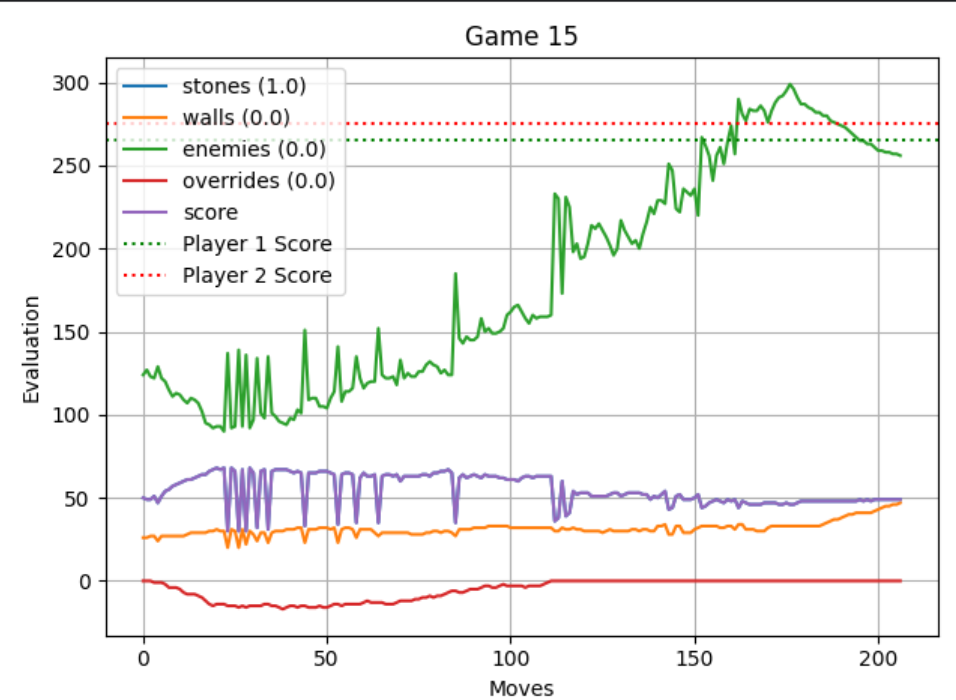
\includegraphics[scale=0.25]{./Graphs/Graph_15.png}
\centering \label{fig1}
\end{figure}

As seen above, using only the Stones heuristic results in a loss. Although the evaluation remained relatively stable, gradually declining toward the end, the point difference to player 2 was not very large. This suggests that while the heuristic provided a reasonably accurate evaluation, it led to poor decisions. The heuristic returns a value between 0 and 100, having a 50 at the end and closely losing is fitting.

\begin{figure}[H]
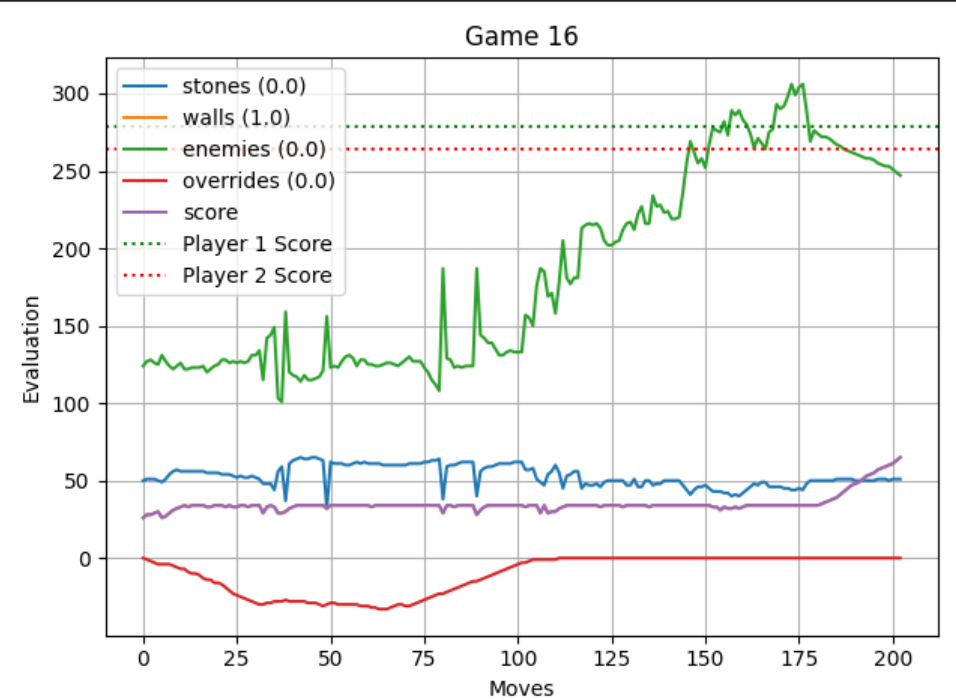
\includegraphics[scale=0.25]{./Graphs/Graph_16.png}
\centering \label{fig1}
\end{figure}

Using only the Walls heuristic proved ineffective. The only noticeable changes occurred during the bomb phase, which significantly increased the number of walls available, due to the bombing. The reason for the poor more or less static behavior of the wall heuristic, is probably the lack of holes on the two test maps, as they had some, but not to many possible walls. 

\begin{figure}[H]
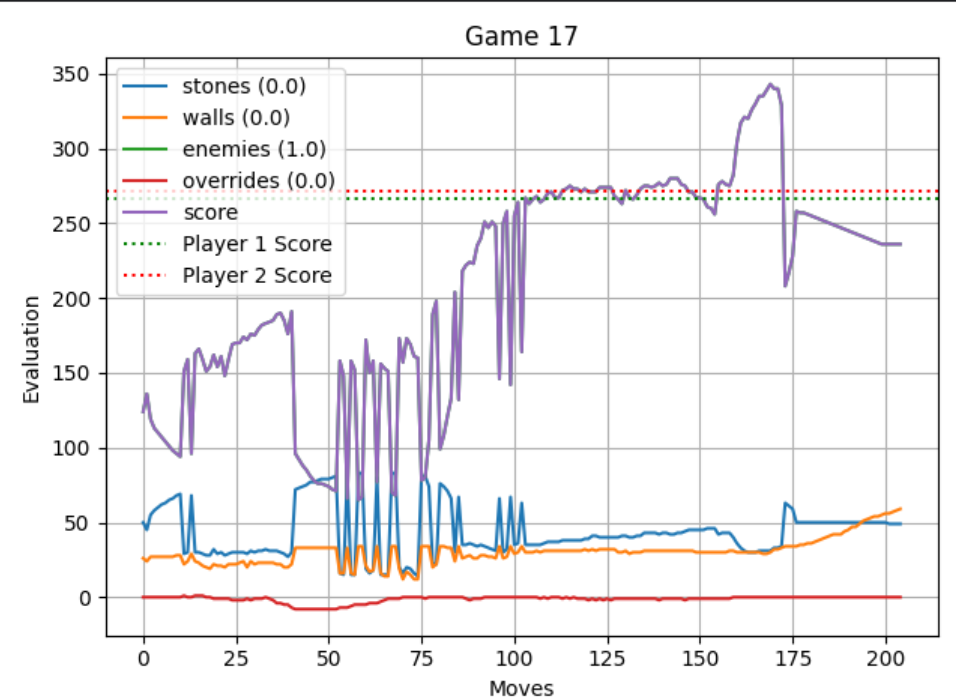
\includegraphics[scale=0.25]{./Graphs/Graph_17.png}
\centering \label{fig1}
\end{figure}

Relying solely on the Enemy adjacency heuristic is problematic. It produces high scores despite losses, furthermore it is incredibly volatile. We can also observe the decrease of enemies in the bombing-phase. This lear us to conclude that the enemy heuristic must be used as a negative heuristic, to discourage to many enemy neighbors.

\begin{figure}[H]
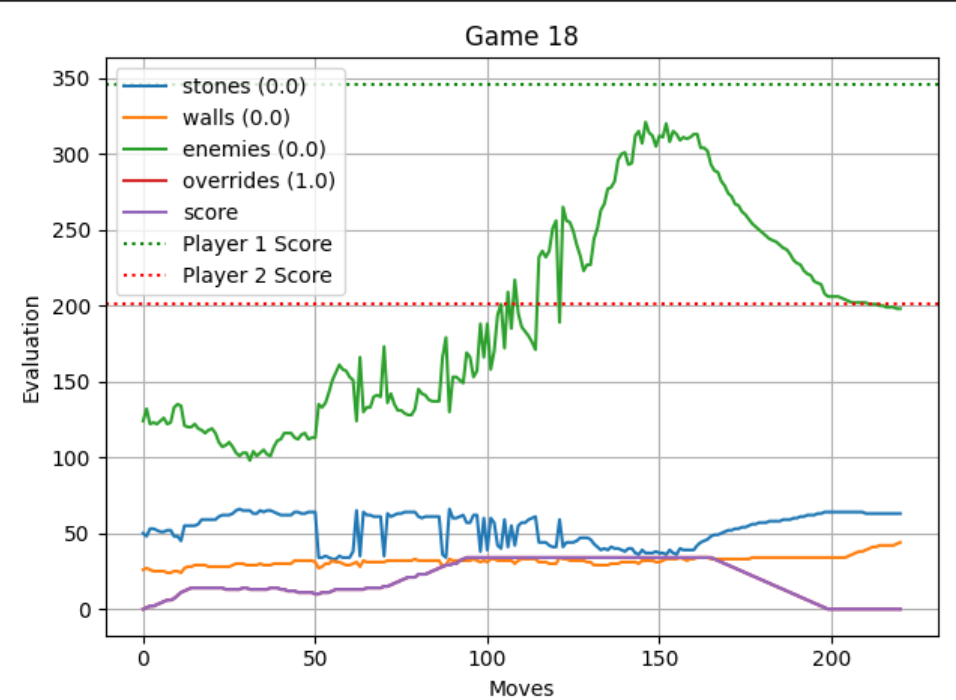
\includegraphics[scale=0.25]{./Graphs/Graph_18.png}
\centering \label{fig1}
\end{figure}

Focusing only on the Override heuristic suggests a strategy of saving override stones early and using them late to reclaim control. This approach resulted in multiple victories.\\
\\
To understand how the heuristics interact with each other, we ran 10 games with roughly chosen weights. Despite the small sample size, we found several interesting patterns.

\begin{figure}[H]
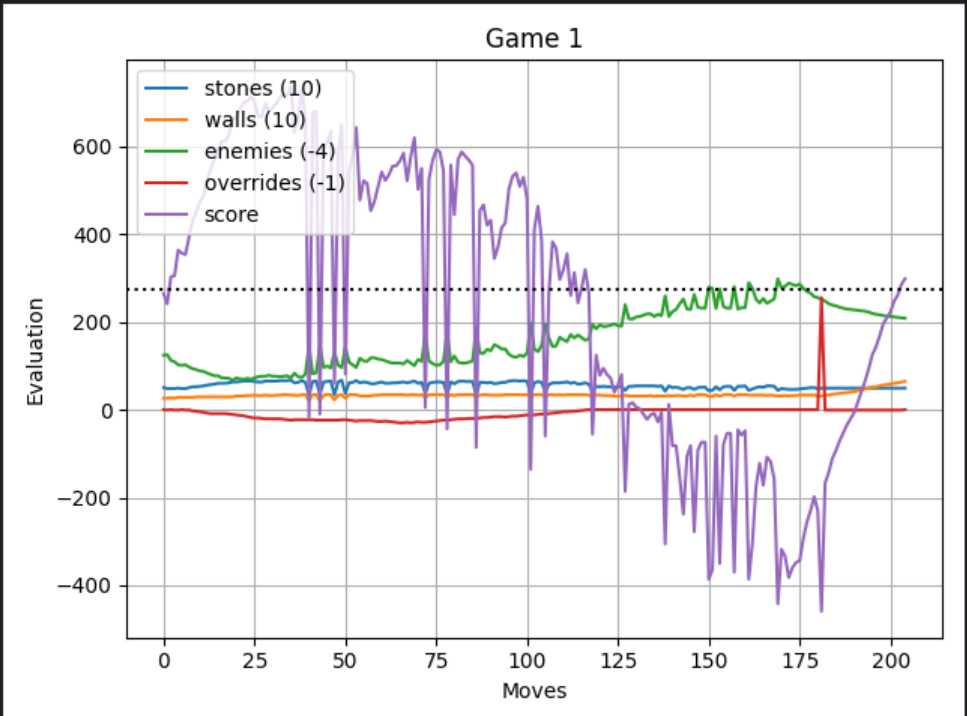
\includegraphics[scale=0.25]{./Graphs/Graph_1.png}
\centering \label{fig1}
\end{figure}

During early tests, we observed a suspicious spike to 255 in the override evaluation during the bomb phase. This led us to discover a byte overflow bug. Although the bug had no significant consequences, it's good that it was resolved.\\
To avoid cluttering this report with too many graphs, we only include key examples here. All other graphs can be found in the Graphs folder of the assignment repository. Throughout all games, we noted the following observations:\\
Stones and Enemies are inversely correlated. When an opponent captures our stones, it increases the number of adjacent enemy pieces. Examples of this behavior can be seen in Games 3, 4, and 5. This results in a double penalty: we lose pieces and gain negatively weighted enemy neighbors.\\
We also noticed that our scores were generally lower than expected. This may be, because we call the evaluation function before our move, so after the opponent has just made a beneficial move for themselves.\\
Furthermore, the score was way more volatile, then we expected. Although events like inversions or choices can drastically change the entire game, we shouldn't or at least don't expect to see such great spikes all the time and in every game.

\begin{figure}[H]
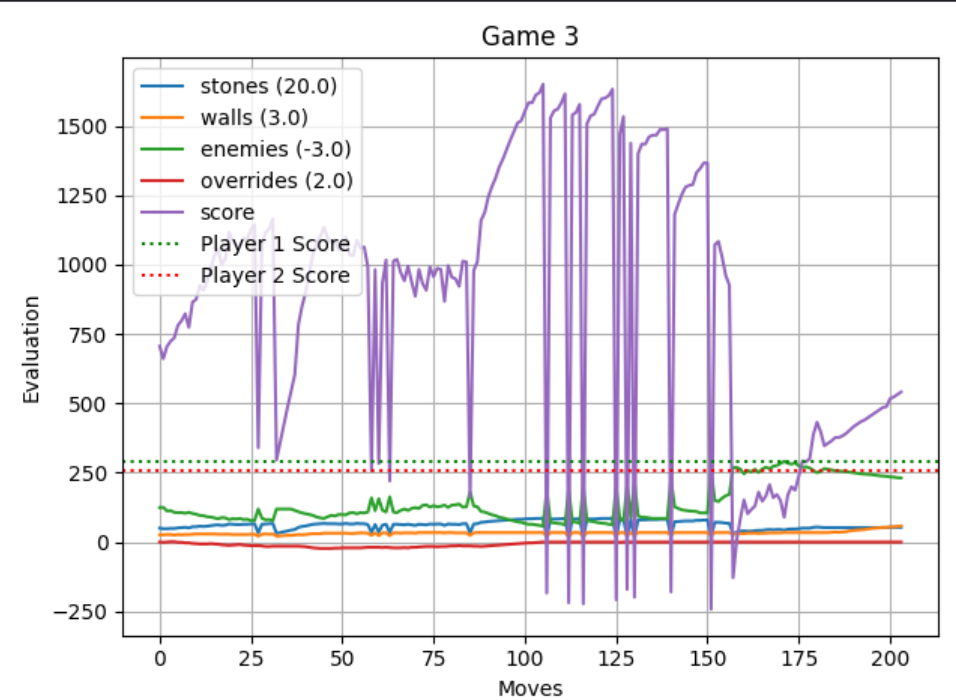
\includegraphics[scale=0.25]{./Graphs/Graph_3.png}
\centering \label{fig1}
\end{figure}

\begin{figure}[H]
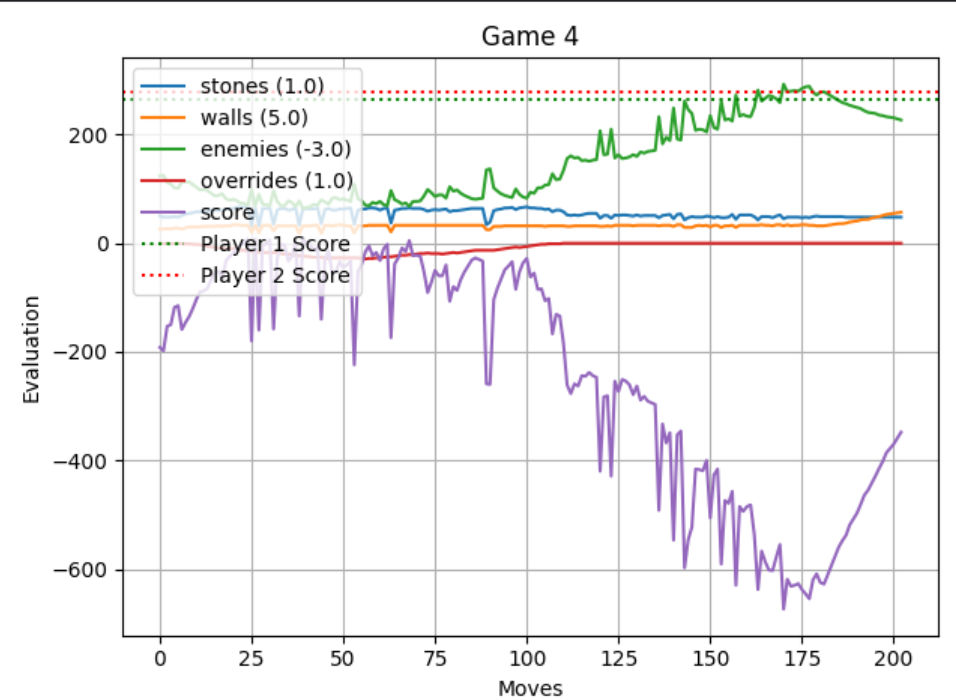
\includegraphics[scale=0.25]{./Graphs/Graph_4.png}
\centering \label{fig1}
\end{figure}

\begin{figure}[H]
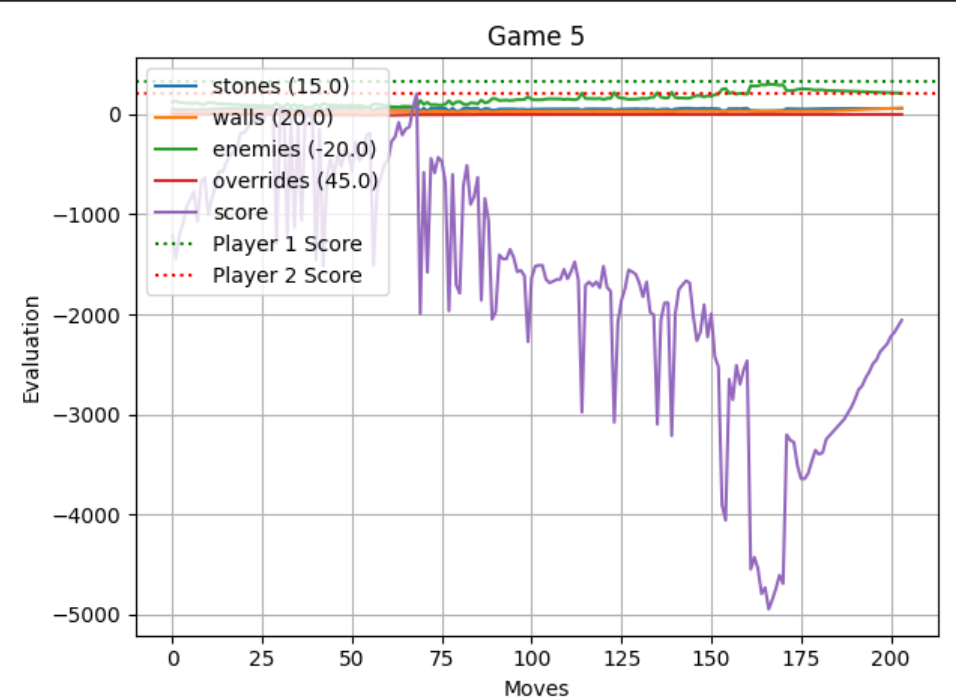
\includegraphics[scale=0.25]{./Graphs/Graph_5.png}
\centering \label{fig1}
\end{figure}

We believe this high volatility in the scores to be especially due to the Enemy heuristic and the large weights used, as stones, walls and overrides were more stable in individual testing and do not move to much or get to large. From this, we learned that smaller weights help reduce fluctuation and that the Enemy heuristic should be assigned a negative weight, as it represents vulnerability to attack.

\begin{figure}[H]
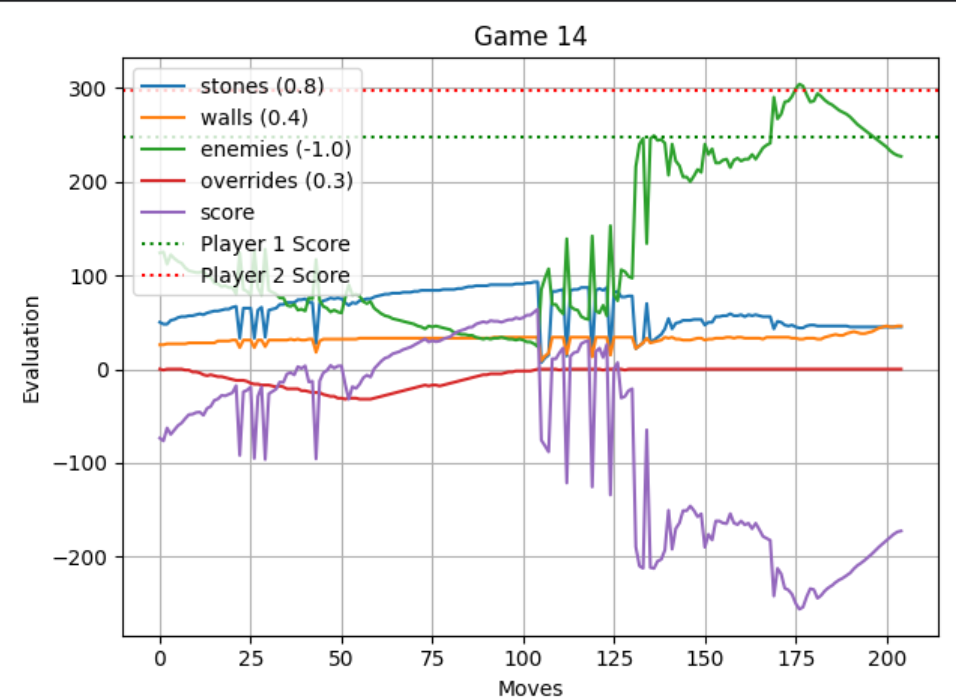
\includegraphics[scale=0.25]{./Graphs/Graph_14.png}
\centering \label{fig1}
\end{figure}

Game 14, although indicating a loss through its score, still ended in a defeat. This suggests the heuristic weights used were not good enough. The problem we identified in game 14, was that enemies was the largest weight. This negatively skewed the entire socre in the end, since enemies always has a great increase in the second half of the game.

\begin{figure}[H]
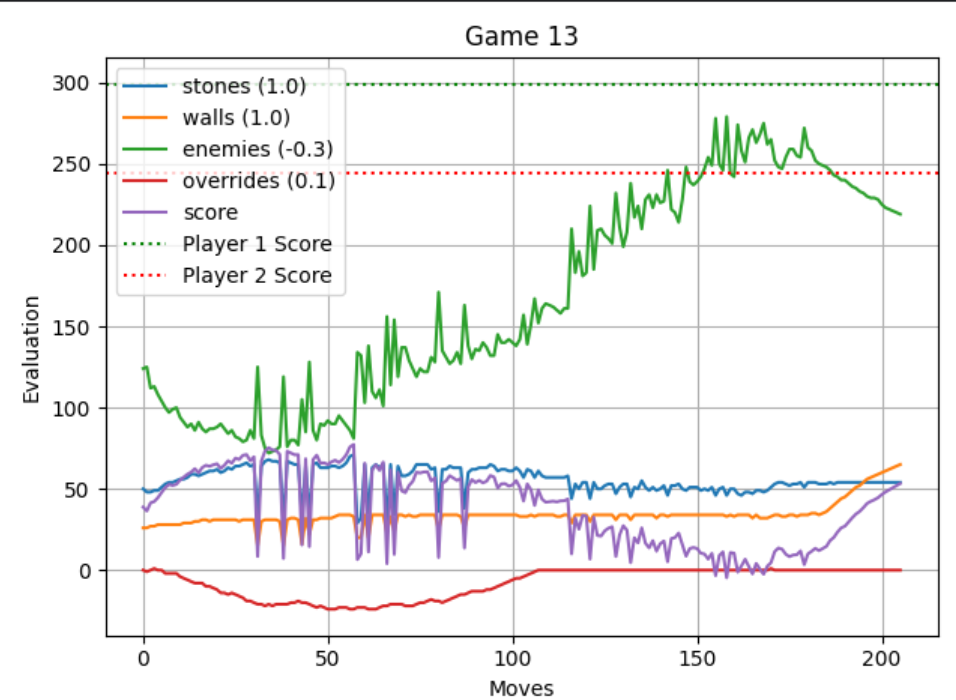
\includegraphics[scale=0.25]{./Graphs/Graph_13.png}
\centering \label{fig1}
\end{figure}

We selected Game 13 as the baseline for future experiments, as it demonstrated a steadily increasing score that culminated in a clear win. Tests with weights similar to those in Game 13 confirmed their effectiveness. We are happy with the 3 to 1 ration between stones and enemies, but still intend to find the best options for overrides and wally.

\begin{figure}[H]
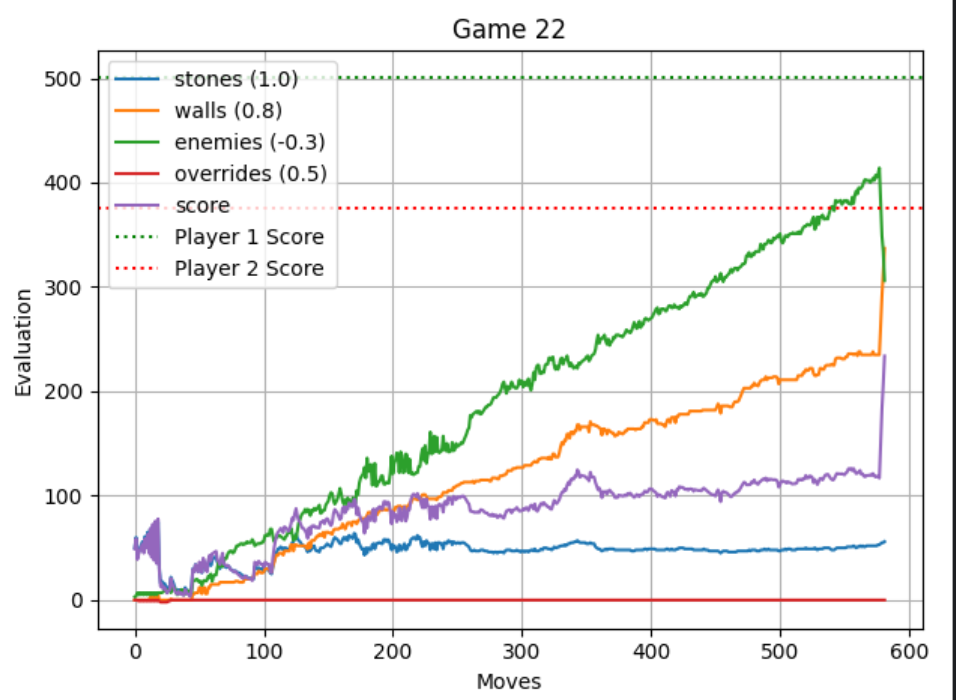
\includegraphics[scale=0.25]{./Graphs/Graph_22.png}
\centering \label{fig1}
\end{figure}

While this evaluation has provided us with a solid baseline, further refinement is planned. Our next steps include:

\begin{enumerate}
    \item Running our client against itself to compare weights more directly.
    \item Using more than two maps to diversify the test environments.
    \item Increasing the number of tests to reduce the impact of outliers.
    \item Analyzing Matchpoint logs to compare predicted and actual scores at the game's end.
    \item As we removed a heuristic, that was not that well thought through and to complex, we need to create a new one.
\end{enumerate}
